\begin{figure}[t]
  \centering
      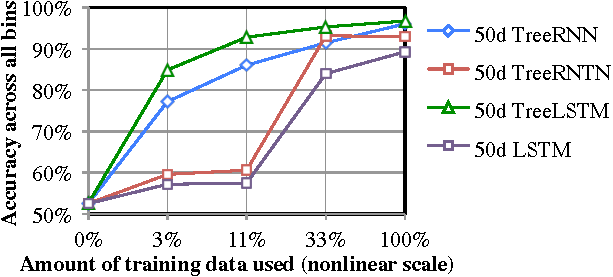
\includegraphics[height=1.3in]{lcc.pdf}
  \caption{Learning curve for the $\le$6 experiment.}
  \label{fig:lc} 
\end{figure}

\section{Results and discussion}\label{sec:discussion}

The results are shown in Figure~\ref{prop-results}. 
The tree models fit the training data well, reaching 99.6, 98.5, and 97.7\% overall accuracy respectively in the $\le$6 setting, with the LSTM underfitting slightly at 94.4\%. 
In that setting, all models generalized well to structures of familiar length, with the tree models all surpassing 97\% on examples of size 4, and the LSTM reaching 94.8\%.
On the longer test sentences, the tree models decayed smoothly in performance across the board, while the LSTM decayed more quickly and more abruptly, with a striking difference in the $\le$4 setting, where LSTM performance falls 10\% from 4 to 5, compared to 4.4\% for the next worse model. However, the LSTM improves considerably with more ample training data in the $\le$6 condition, showing only a 3\% drop and generalization results better than the best model's in the $\le$3 setting.

All four models robustly beat the simple baselines reported in Bowman et al.: the most frequent class occurs just over 50\% of the time and a neural bag of words model does reasonably on the shortest examples but falls below 60\% by bin~4.

The learning curve (Figure~\ref{fig:lc}) suggests that additional data is unlikely to change these basic results, though the disparity in performance at the 11\% level is striking: the LSTM sequence model and the TreeRNTN (the model with the most parameters by far) lag far behind the other two.

\section{Conclusion}

We find that all four models can exploit a recursively defined language to interpret sentences with complex unseen structures, and that tree models' biases allow them to learn to do this more effectively from less data.
We interpret these results as evidence that both tree and sequence architectures can play valuable roles in the construction of sentence models over data with recursive syntactic structure: tree architectures provide an explicit bias that makes it possible to learn from relatively small and impoverished data sets, while sequence-based architectures can solve the same problems---given sufficient data---without being constrained by this bias. Finally, we suggest that, because of the well-supported linguistic claim that the kind of recursive structure that we study here is key to the understanding of real natural languages, there is likely to be value in developing sequence models that can more efficiently exploit this structure without fully sacrificing the flexibility that makes them succeed.

